\section{Software architecture}

\begin{figure}
  \centering
  \makebox[\textwidth][c]{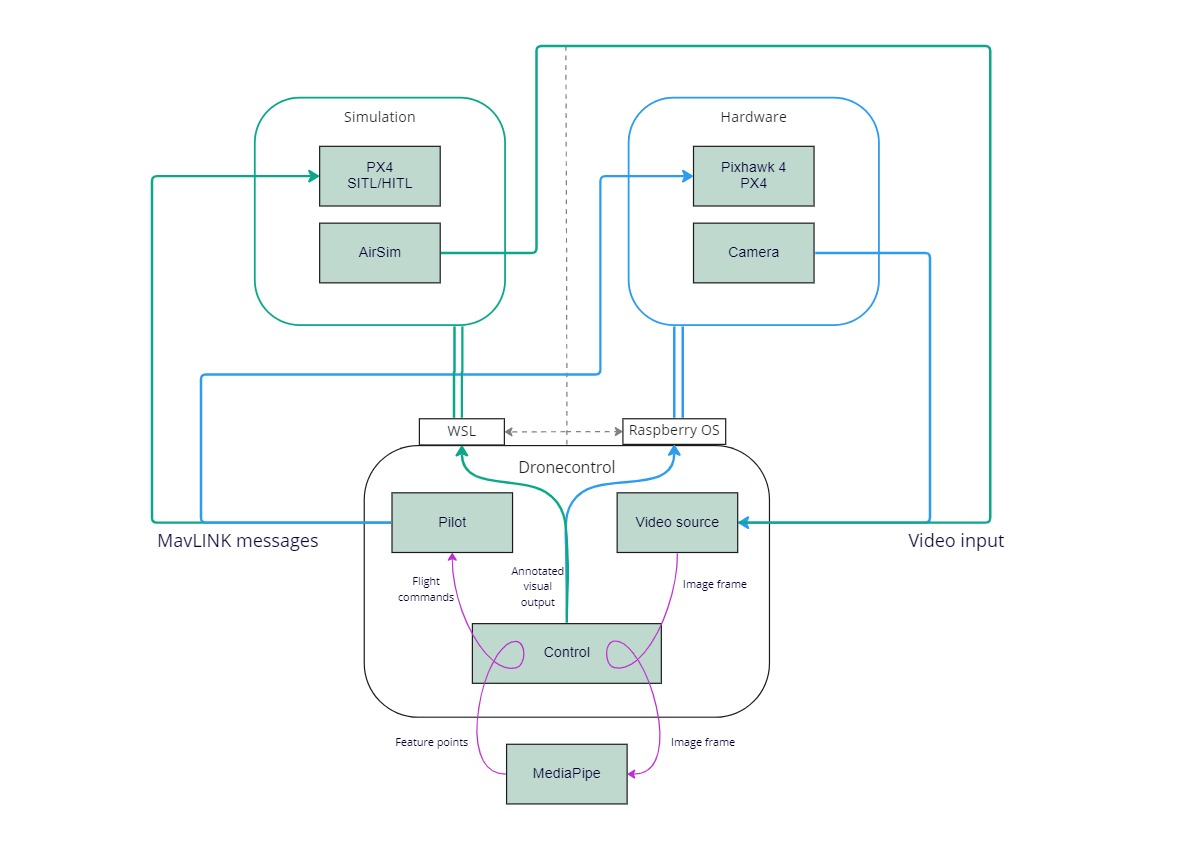
\includegraphics[width=1.4\textwidth, keepaspectratio]{img/software-arch.jpg}}
  \caption{Structure of the DroneVisionControl application main modules (green background) and its interactions with the external components (white background). The information flow is shown in purple arrows for internal communication, green arrows for the simulation environment and blue arrows for hardware interactions.}
\label{fig:soft-arch}
\end{figure}

This section presents the software architecture of the DroneVisionControl application. Except when noted as an external library, all the functionality described has been developed specifically for this project. The complete codebase is located in a GitHub repository\footnote{\url{https://github.com/l-gonz/tfg-giaa-dronecontrol}}.
Figure \ref{fig:soft-arch} illustrates the main modules of the designed software and their interactions with external libraries. The application comprises three fundamental parts: the \textbf{pilot module}, responsible for sending instructions to the flight controller and receiving position and state information through the \texttt{mavsdk} library; the \textbf{video source module}, which handles image retrieval from various sources and performs necessary image analysis processing; and the \textbf{control module}, which facilitates interaction between the other two modules to convert pixel information into position points using the \texttt{mediapipe} library, and further into instructions for the pilot.

In the upper part of the diagram in Figure \ref{fig:soft-arch}, the flow of information between the DroneVisionControl application and the external systems is depicted. Green lines represent the path in a simulated workflow, while blue lines indicate the alternative path for a system with actual quadcopter hardware. Purple arrows indicate the input/output of each module within the developed application and how they interconnect. Additionally, smaller utilities have been developed to test the interaction between systems and calibrate different aspects of the control behaviour. These utilities are described in sections \ref{subsec:cam-tool} and \ref{subsec:pid-tools}. A user manual with all the options available in the application can be found in Appendix \ref{app:cli}.

\subsection{Pilot module}
\label{subsec:pilot-module}

The pilot module\footnote{\url{https://github.com/l-gonz/tfg-giaa-dronecontrol/blob/main/dronecontrol/common/pilot.py}} serves the purpose of providing access to the rest of the application for sending and receiving messages from the PX4 controller through the external MAVSDK library. This library offers a simple asynchronous API for managing one or more vehicles, allowing programmatic access to vehicle information, telemetry, and control over missions, movements, and other operations. The integration of MAVSDK with the pilot module utilizes the Python library \texttt{asyncio} \cite{asyncio}, which enables running coroutines in parallel while waiting for messages provided through MAVLink communication.

To interact with the MAVSDK library, all calls need to be written as async functions that await the result of one or more polls to the flight stack. The \texttt{asyncio} library provides support for writing concurrent code using the \texttt{async/await} syntax, serving as a foundation for various Python asynchronous frameworks used for high-performance network and web servers, database connection libraries, and distributed task queues. It offers a set of high-level APIs to run Python coroutines concurrently and grants complete control over their execution.

The pilot module, integrating MAVSDK and \texttt{asyncio}, provides functionality to establish a connection to a PX4 vehicle through a physical serial address or a UDP endpoint.
During this connection phase, the module will poll for internal information from the flight controller to decide when the system is ready to receive instructions.
The MAVSDK library exposes telemetry and other state information through asynchronous generators, defined in Python as a convenient way to retrieve data asynchronously. These are accessed with the \texttt{async\ for} syntax.

The pilot module implements many basic operations that can be executed in the flight controller, along with error handling and safety checks. These operations include takeoff, landing, return home, and manipulating the vehicle's flying velocity directly by providing speeds in body coordinates. These commands can be sent to a vehicle once a connection has been established. 
To enable direct control of the vehicle's velocity, a special flight mode defined by PX4, called Offboard mode \cite{offboard-mode}, is required (not related to the offboard configuration described in Section \ref{subsec:offboard}). Offboard mode primarily controls vehicle movement and attitude, adhering to setpoints provided through MAVSDK. This mode relies on position or pose/attitude information available to the flight controller, such as through a gyroscope and a GPS antenna. 
For safety purposes, this mode requires a constant stream of commands to be maintained.
If the message rate falls below 2Hz or the connection is lost, the vehicle will come to a halt and, after a timeout, attempt to land or perform other failsafe actions based on the configured parameters.
This behaviour is handled internally by the MAVSDK library and made available to the application by the pilot module through a \texttt{toggle\_offboard\_mode} function.


As an additional feature, the pilot module also implements an asynchronous queue that can be used to execute actions sequentially. The queue is periodically polled to search for newly added commands to execute, ensuring that each action waits until the previous one has finished and the vehicle is in the desired state before starting the next action. Using this queue is optional and depends on the specific behaviour desired from the control solution. All pilot commands can either be executed immediately, interrupting whichever action is being executed at that time, or be added to the queue to be executed at a later point.


By encapsulating the functionality of sending commands and receiving information from the flight controller, the pilot module provides a robust interface for controlling the vehicle's behaviour and enables seamless integration with other components of the application.


\subsection{Video source module}
\label{subsec:viz-source-module}

The video source module\footnote{\url{https://github.com/l-gonz/tfg-giaa-dronecontrol/blob/main/dronecontrol/common/video_source.py}} aims to provide a collection of classes to retrieve images from different sources in a manner that allows easy interchangeability without affecting the rest of the application. 
This design facilitates testing and adaptability to various environments. Three classes of video sources have been implemented: file, simulator, and camera, all of which inherit from the \texttt{VideoSource} class, as shown in the diagram in Figure \ref{fig:video-source-inheritance}.

\begin{figure}
  \centering
  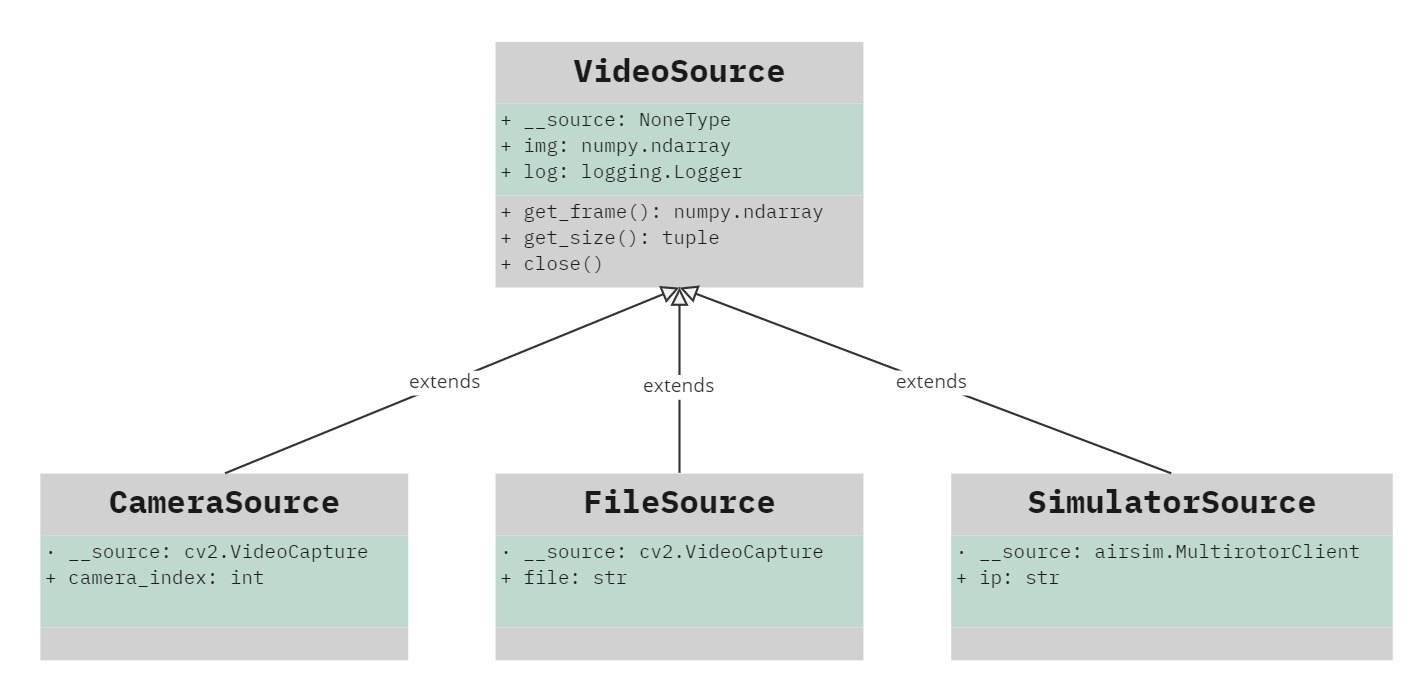
\includegraphics[width=\textwidth, keepaspectratio]{img/uml-video-source.jpg}
  \caption{Diagram of inheritance on the video source classes available to retrieve image data.}
  \label{fig:video-source-inheritance}
\end{figure}

The \texttt{FileSource} class can open a video file stored on the companion computer and provide frames sequentially until the video is completed. This feature enables the replaying image detection algorithms on previously captured videos using the camera tool described in Section \ref{subsec:cam-tool}. The \texttt{CameraSource} class can access a physical camera connected to the computer running the application via USB and provide real-time captured frames. Both the file and camera sources leverage OpenCV's video capture utilities to handle file operations and camera drivers.

The \texttt{SimulatorSource} utilizes AirSim's Python library, \texttt{airlib}, to communicate with the simulator and retrieve images from a camera object attached to the vehicle model in Unreal Engine. It establishes an automatic connection to the simulator via \texttt{localhost}, but it can also be initialized with an IP address to connect to a simulator running on a different computer within the local network. This is particularly useful when the DroneVisionControl runs inside a Linux subsystem (WSL) and the simulator operates on the host Windows system.

\subsection{Vision control module}
\label{subsec:control-module}

The control module encompasses the main logic of the application and is responsible for converting raw images obtained from the video source into commands for the pilot module. Two different types of control solutions have been implemented. The first one is the proof-of-concept control solution described in Section \ref{sec:hands}, operating in the offboard configuration outlined in Section \ref{subsec:offboard}. Its purpose is to translate predefined hand gestures into movement commands for the aerial vehicle. This solution facilitates testing the interaction between all system components in a contained environment by situating the controlling computer outside of the vehicle. The second control system is a follow mechanism, described in Section \ref{sec:follow}, which aims to mimic real-life scenarios where the control algorithms and camera reside onboard the vehicle. It tracks the location of a person detected in the images captured from the drone's perspective and uses that information to calculate velocities necessary for following and keeping the person centred in the drone's view.

Both solutions follow a similar process that can be divided into three steps:
\begin{enumerate}
    \item The image is sent to the MediaPipe computer-vision third-party library, described in Section \ref{subsec:mediapipe}, which extracts the required features from the image in the form of 2D coordinates. In the hand solution, the coordinates match the features of a detected hand and in the follow solution, the features of a person, as shown in Figures \ref{fig:hand-landmarks} and \ref{fig:pose-landmarks}, respectively.
    \item Various calculations specific to each solution are applied to these coordinates. In the hand solution, gestures are extracted from the coordinates through vector calculations, and in the follow solution, a bounding box is drawn around the person to determine its relative position on the field of view.
    \item The commands sent to the pilot module are determined based on the input calculated from the coordinates. In the hand solution, each gesture is mapped to a single command, and in the follow solution, velocity commands are extracted from the bounding box position through a PID controller.
\end{enumerate}

Captured images, detected features and calculated results are communicated to a simple \acrshort{gui}, drawn with the help of the OpenCV library. This interface shows the user all the necessary information about the current state of the running application. Sections \ref{sec:hands} and \ref{sec:follow} provide further explanations of the control modules used in the two different solutions developed.

\subsection{Camera-testing tool}
\label{subsec:cam-tool}

In addition to the main modules, several utilities have been included in the DroneVisionControl program to facilitate the development and testing processes of the control solutions. The first tool is available in the \texttt{test\_camera} module\footnote{\url{https://github.com/l-gonz/tfg-giaa-dronecontrol/blob/main/dronecontrol/tools/test_camera.py}} and can be accessed through the command \texttt{dronevisioncontrol tools test-camera}. This tool serves multiple purposes, including testing the connection between the computer, the flight stack, and the camera without needing to attach any self-guided control mechanism. It also allows evaluation of the performance of the MediaPipe hand and pose machine learning solutions on real-time images. Additionally, it enables image capture and video recording from a live camera feed for subsequent analysis. 

The test tool can be configured through command-line options to use any of the three available video sources (camera, simulator, or video file), connect to a hardware or simulated PX4 flight controller by specifying a connection string or IP, and run on any system acting as a companion computer. Computer vision can optionally be enabled to process incoming images using hand or pose recognition software. While the tool is running, basic commands such as takeoff, landing, or movement along any direction can be sent to a connected vehicle using the keyboard. Appendix \ref{app:cli} provides a comprehensive breakdown of all the tool's options.

This tool will be used extensively during the tests carried out in Chapter \ref{chap:validation} to validate individual application components in different scenarios without involving complex control mechanisms.
